% !TeX root = proposal.tex
\chapter{Recommending Privacy Preference for General IoT}
In this chapter, we present the work completed to date in the areas of recommending privacy preference for general IoT, including the data-driven design, the dataset that we use, the inspection of users' behaviors using statistical analyses, prediction of users' behaviors using machine learning techniques, and the privacy-setting prototypes that we create based on both statistical and machine learning results.

\section{Data-driven design}
What design process allows us to develop a usable privacy-setting interface for IoT? The development of usable privacy interfaces commonly relies on user studies with existing systems. However, this method is not possible in our IoT control scenario, because the Intel control framework has yet to be implemented~\cite{chow2015hci}. We therefore develop and employ a \emph{data-driven design} methodology, leveraging an existing dataset collected by Lee and Kobsa~\cite{lee2016understanding}, who asked users whether they would allow or deny IoT devices in their environment to collect information about them. We use this dataset in two phases. 

In our first phase, we develop a ``layered'' settings interface, where users make a decision on a less granular level (e.g., whether a certain recipient is allowed to collect their personal information or not), and only move to a more granular decision (e.g., what types of information this recipient is allowed to collect) when they desire more detailed control. This reduces the complexity of the decisions users have to make, without reducing the amount of control available to them. We use statistical analysis of the Lee and Kobsa dataset to decide which aspect should be presented at the highest layer of our IoT privacy-setting interface, and which aspects are relegated to subsequently lower layers.

In our second phase, we develop a ``smart'' default setting, which preempts the need for many users to manually change their settings~\cite{smith2013choice}. However, since people differ extensively in their privacy preferences~\cite{olson2005study}, it is not possible to achieve an optimal default that is the same for everyone. Instead, different people may require different settings. Outside the field of IoT, researchers have been able to establish distinct clusters or ``profiles'' based on user behavioral data~\cite{knijnenburg2013dimensionality, olson2005study, wisniewski2017making}. We perform machine learning analysis on the Lee and Kobsa dataset to create a similar set of ``smart profiles'' for our IoT privacy-setting interface.

The remainder of this paper is structured as follows: We first summarize previous work on privacy in IoT scenarios, and describe the structure of the Lee and Kobsa~\cite{lee2016understanding} dataset. We then \emph{inspect} users' behaviors using statistical analysis. Next, we \emph{predict} users' behaviors using machine learning methods. We subsequently present a set of prototypes for an IoT privacy-setting interface. Finally, we conclude with a summary of our proposed procedure and the results of our analysis.

\subsection{Dataset}
This study is based on a dataset collected by Lee and Kobsa~\cite{lee2016understanding}. A total of 2800 scenarios were presented to 200 participants (100 male, 99 female, 1 undisclosed) through Amazon Mechanical Turk. Four participants were aged between 18 and 20, 75 aged 20--30, 68 aged 30--40, 31 aged 40--50, 20 aged 50--60, and 2 aged $>$ 60. 

Each participant was presented with 14 scenarios describing a situation where an IoT device would collect information about the participant. Each scenario was a combination of five contextual parameters (Table~\ref{tab:parameter}), manipulated at several levels using a mixed fractional factorial design that allowed us to test main effects and two-way interactions between all parameters.

For every scenario, participants were asked a total of 9 questions. Our study focuses on the \textbf{allow/reject} question: ``If you had a choice to allow/reject this, what would you choose?'', with options ``I would allow it'' and ``I would reject it''. We also used participants' answers to three attitudinal questions regarding the scenario:
\begin{itemize}
	\item \textbf{Risk:} How risky or safe is this situation? (7pt scale from ``very risky'' to ``very safe'')
	\item \textbf{Comfort:} How comfortable or uncomfortable do you feel about this situation? (7pt scale)
	\item \textbf{Appropriateness:} How appropriate do you consider this situation? (7pt scale)
\end{itemize}

\begin{table*}
	\caption{Parameters used in the experiment. Example scenarios: \\\emph{``A device of a friend records your video to detect your presence. This happens continuously, while you are at someone else's place, for your safety.''}\\\emph{``A government device reads your phone ID to detect your identity. This happens once, while you are in a public place (e.g. on the street), for health-related purposes.''}}
	\label{tab:parameter}
	\begin{tabular}{l | l}
		\hline
		\textbf{Parameter} & \textbf{Levels} 	 \\ \hline
		\multirow{7}{9.5em}{Who\\\rule{0pt}{4ex}\emph{The entity collecting the data}}		& 1. Unknown \\
		& 2. Colleague							 \\
		& 3. Friend								 \\
		& 4. Own device							 \\
		& 5. Business 							 \\
		& 6. Employer 							 \\
		& 7. Government							 \\ \hline
		\multirow{24}{9.5em}{What\\\rule{0pt}{4ex}\emph{The type of data collected and (optionally) the knowledge extracted from this data}}	& 1. PhoneID	\\	
		& 2. PhoneID$>$identity				\\	
		& 3. Location						\\	
		& 4. Location$>$presence			\\	
		& 5. Voice							\\	
		& 6. Voice$>$gender					\\	
		& 7. Voice$>$ age 					\\	
		& 8. Voice$>$identity				\\	
		& 9. Voice$>$presence				\\	
		& 10. Voice$>$mood					\\	
		& 11. Photo							\\	
		& 12. Photo$>$gender				\\	
		& 13. Photo$>$age  \\
		& 14. Photo$>$identity	 \\
		& 15. Photo$>$presence 	 \\
		& 16. Photo$>$mood 	 \\
		& 17. Video	 \\
		& 18. Video$>$gender	 \\
		& 19. Video$>$age 		 \\
		& 20. Video$>$presence 	 \\
		& 21. Video$>$mood 	 \\
		& 22. Video$>$looking at	 \\
		& 23. Gaze	 \\
		& 24. Gaze$>$looking at	 \\ \hline
		\multirow{4}{9.5em}{Where\\\rule{0pt}{4ex}\emph{The location of the data collection}}	& 1. Your place		\\
		& 2. Someone else's place		\\				
		& 3. Semi-public place (e.g. restaurant) \\
		& 4. Public space (e.g. street) \\ \hline
		\multirow{6}{9.5em}{Reason\\\rule{0pt}{4ex}\emph{The reason for collecting this data}} & 1. Safety	\\
		& 2. Commercial						\\
		& 3. Social-related	\\
		& 4. Convenience \\
		& 5. Health-related \\
		& 6. None \\ \hline
		\multirow{2}{9.5em}{Persistence} & 1. Once \\
		& 2. Continuously \\ 
		\emph{Whether data is collected once or continuously} & \\ \hline
	\end{tabular}
\end{table*}



In this section we analyze how users' behavioral intentions to allow or reject the information collection described in the scenario are influenced by the scenario parameters. In line with classic attitude-behavior models~\cite{ajzen1977attitude}, we also investigate whether users' attitudes regarding the scenario---their judgment of risk, comfort, and appropriateness---mediate these effects. This mediation analysis~\cite{baron1986moderator} involves the following test:
\begin{itemize}
\item \textbf{Test 1:} The effect of the scenario parameters (who, what, where, reason, persistence) on participants' attitudes (risk, comfort, appropriateness).
\item \textbf{Test 2:} The effect of participants' attitudes on their behavioral intentions (the allow/reject decision).
\item \textbf{Test 3:}  The effect of the parameters on behavioral intentions, controlling for attitudes.
\end{itemize}

If tests 1 and 2 are significant, and test 3 reveals a substantial reduction in conditional direct effect (compared to the marginal effect), then we can say that the effects of the scenario parameters on participants' behavioral intention are mediated by their attitudes. Moreover, if the conditional direct effect is (close to) zero, then the effects are fully (rather than partially) mediated.

\subsection{Scenario Parameters and Attitude}\label{subsec:attitude}
\subsubsection{ANOVA Test of Main Effects}
To understand the effect of the scenario parameters on participants' attitudes, we created a separate \textit{linear mixed effects regression} (\textit{lmer}) model with a random intercept (to account for repeated measures on the same participant) for each dependent variable (risk, comfort, appropriateness), using the scenario parameters as independent variables. We employed a forward stepwise procedure, adding the strongest remaining parameter into the model at each step and comparing it against the previous model. Table~\ref{tab:anovaEffect} shows that all parameters except \textbf{where} have a significant effect on each of the attitudes.

\subsubsection{Post-hoc Comparisons}
We also conducted Tukey post hoc analyses to better understand how the various values of each parameter influenced the attitudes. \textbf{Where} was excluded from these analyses, as it did not have an overall significant effect. Some key findings of these post hoc analyses are:

\begin{table}
\centering
\caption{Effect of scenario on attitudes. Each model builds upon and is tested against the previous.}
\label{tab:anovaEffect}
\begin{tabular}{ l | r | r | r}
\hline
Model &	$\chi^2$ &	$df$ & $p$-value \\ \hline
$risk\sim(1|sid)$ &				 &			 &						\\
+who &				315.37 &	6 &			$<$ .0001 		\\
+what &			67.74 &		23 &		$<$ .0001 		\\
+reason & 			15.65 &		5 &		.0079 			\\
+persistence &		9.95 &		1 &		.0016 			\\
+where	&			7.47 &		3 &		.0586 			\\
+who:what &		166.47 &	138 &	.0050			\\
\hline
Model &	$\chi^2$ &	$df$ & $p$-value \\ \hline
$comfort\sim(1|sid)$ & 			 &			&	 					\\
+who &				334.06 &	6 &			$<$ .0001 		\\
+what &			83.24 &		23 &		$<$ .0001 		\\
+reason &			18.68 &		5 &			.0022 		\\
+persistence &		14.73 &		1 &			.0001 		\\
+where &			3.25 &		3 &			.3544 		\\
+who:what &		195.07 &	138 &		.0001			\\
\hline
Model &	$\chi^2$ &	$df$ & $p$-value \\ \hline
$appropriateness\sim(1|sid)$ &	 &		 &						\\
+who &				315.77 &	6 &			$<$ .0001 		\\
+what &			72.87 &		23 &		$<$ .0001 		\\
+reason &			23.27 &		5 &			.0003 		\\
+persistence &		8.97 &		1 &			.0027 		\\
+where &			5.46 &		3 &			.1411 		\\
+who:what &		214.61 &	138 &		$<$ .0001			\\
\hline
\end{tabular}
\end{table}

\textbf{Who:} Participants perceive more \emph{risk} when the recipient of the information is `unknown' than for any other recipient ($d$ range = [0.640, 1.450] and all $p$s~$<$~.001, except for `government': $d=0.286$, $p < .05$). `Government' is the next most risky recipient ($d$ range = [0.440, 1.190], all $p$s~$<$~.001). Participants consider their `own device' the least risky ($d$ range = [0.510, 1.450], all $p$s~$<$~.001). Similar patterns were found for \emph{comfort} and \emph{appropriateness}.

\textbf{Reason:} Participants were more \emph{comfortable} disclosing information for the purpose of `safety' than for any other reason except `health' ($d$ range = [0.230, 0.355], all $p$s~$<$~.05). They also believe that disclosing information for the purpose of `health' or `safety' is more \emph{appropriate} than for `social' or `commercial' purposes ($d$ range = [0.270, 0.310], all $p$s~$<$~.05).

\textbf{Persistence:} Participants were more \emph{comfortable}, found it more \emph{appropriate}, and less \emph{risky} to disclose their information `once' rather than `continuously' ($d = 0.146$, $p < .01$).

\textbf{What:} This parameter has a large number of values, so we decided to selectively test planned contrasts instead of post-hoc tests. We first compared different mediums (voice, photo, video) regardless of what is being inferred:
\begin{itemize}
\item Participants were significantly more \emph{comfortable} with `voice' than `video' ($d = 0.260$, $p = .005$), and found `voice' less \emph{risky} ($d = -0.239$, $p = .005$) and more \emph{appropriate} ($d = 0.217$, $p = .015$) than `video'.
\item Participants were significantly more \emph{comfortable} with `voice' than `photo' ($d=0.201$, $p = .007$) and found `voice' more \emph{appropriate} than `photo' ($d = 0.157$, $p$~$=$~$.028$). There was no significant difference in terms of \emph{risk} ($p = .118$).
\item No differences were found between `photo' and `video' in terms of \emph{risk} ($p = .24$), \emph{comfort} ($p = .35$) and \emph{appropriateness} ($p = .26$).
\end{itemize}

We also compared different inferences (e.g. age, gender, mood, identity) across mediums. The following planned contrasts were significant (all others were not):
\begin{itemize}
\item Participants were significantly more \emph{comfortable} ($d$~$=$~$0.363$, $p = .028$) and found it more \emph{appropriate} ($d = 0.371$, $p = .018$) to reveal their `age' rather than their `identity'.
\item Participants were significantly more \emph{comfortable} ($d$~$=$~$0.363$, $p= .008$) and found it more \emph{appropriate} ($d = 0.308$, $p = .024$) to reveal their `presence' rather than their `identity'.
\end{itemize}

\subsubsection{Interaction effects}
We also checked for two-way interactions between the scenario parameters. The only significant interaction effect observed was between \textbf{who} and \textbf{what}. The last line of each section in Table~\ref{tab:anovaEffect} shows the results of adding this interaction to the model. Due to space concerns, we choose not to address the post-hoc analysis of the $7 * 24 = 168$ specific combinations of who and what.

\subsection{Attitude and Behavioral intention}
To test the effects of participants' attitudes on their allow/reject decision, we ran a \emph{generalized linear mixed effects regression} (\emph{glmer}) with a random intercept and a logit link function to account for the binary dependent variable.
We found significant effects of all the three attitudes on participants' allow/reject decision (see Table~\ref{tab:mediationANOVA}). Each 1-point increase in \textbf{risk} results in a 4.04-fold decrease in the odds that the scenario will be allowed ($p < .0001$). Each 1-point increase in \textbf{comfort} results in a 5.04-fold increase ($p < .0001$), and each 1-point increase in \textbf{appropriateness} results in a 3.47-fold increase ($p < .0001$).

\subsection{Mediation Analysis}
The bottom half of Table~\ref{tab:mediationANOVA} shows the \emph{conditional} effects of the significant parameters (who, what, reason, persistance) on participants' allow/reject decision, controlling for attitude. \textbf{Who} and \textbf{what} are no longer significant; these effects are thus fully mediated by attitude. The effects of \textbf{reason} and \textbf{persistance} are still significant, but smaller than the marginal effects (i.e., without controlling for attitude, see Table~\ref{tab:marginalANOVA})---their $\chi^2$s are reduced by 12\% and 39\%, respectively. This means that the mediation effect was substantial in all cases. The final mediation model is displayed in Figure~\ref{fig:mediationAllow}.


\begin{table}
\centering
\caption{Effect of attitudes and scenario on allow/reject.}
\label{tab:mediationANOVA}
\begin{tabular}{ l | r | r | r | r }
\hline
Model & OR	&	\textbf{$\chi^2$} & $df$ & $p$-value 	\\ \hline
$allow\sim(1 | sid)$ &	&		  &	    &				\\
+risk &				0.25 &	1005.24  &    1 &		$<$ .0001 \\
+comfort &			5.04 &	723.27  &     1 &		$<$ .0001 \\
+appropriateness &	3.47 &	128.17  &	  1 & 		$<$ .0001 \\ \hline
+who &					&	8.80	& 	  6 & 		.1851 	\\
+what &					&	26.07 &	  	 23 &		.2976 	\\
+reason &				&	19.33 & 	  5 & 		.0017	\\
+persistence &			&	12.69 &	 	  1 & 		.0004 	\\
\hline
\end{tabular}
\end{table}

\begin{table}
\centering
\caption{Effect of scenario on allow/reject, \emph{not} controlling for attitudes.}
\label{tab:marginalANOVA}
\begin{tabular}{ l | r | r | r }
\hline
Model &	$\chi^2$ & $df$ & $p$-value 	\\ \hline
$allow\sim(1 | sid)$ &		  	&	    &				\\
+who &					221.36	& 	  6 & 		$<$ .0001 	\\
+what &					78.55 &		  23 &		$<$ .0001 	\\
+reason &				21.95 & 	  5 & 		  .0005		\\
+persistence &			20.64 &		  1 & 		$<$ .0001 	\\
\hline
\end{tabular}
\end{table}

\begin{figure}
\centering
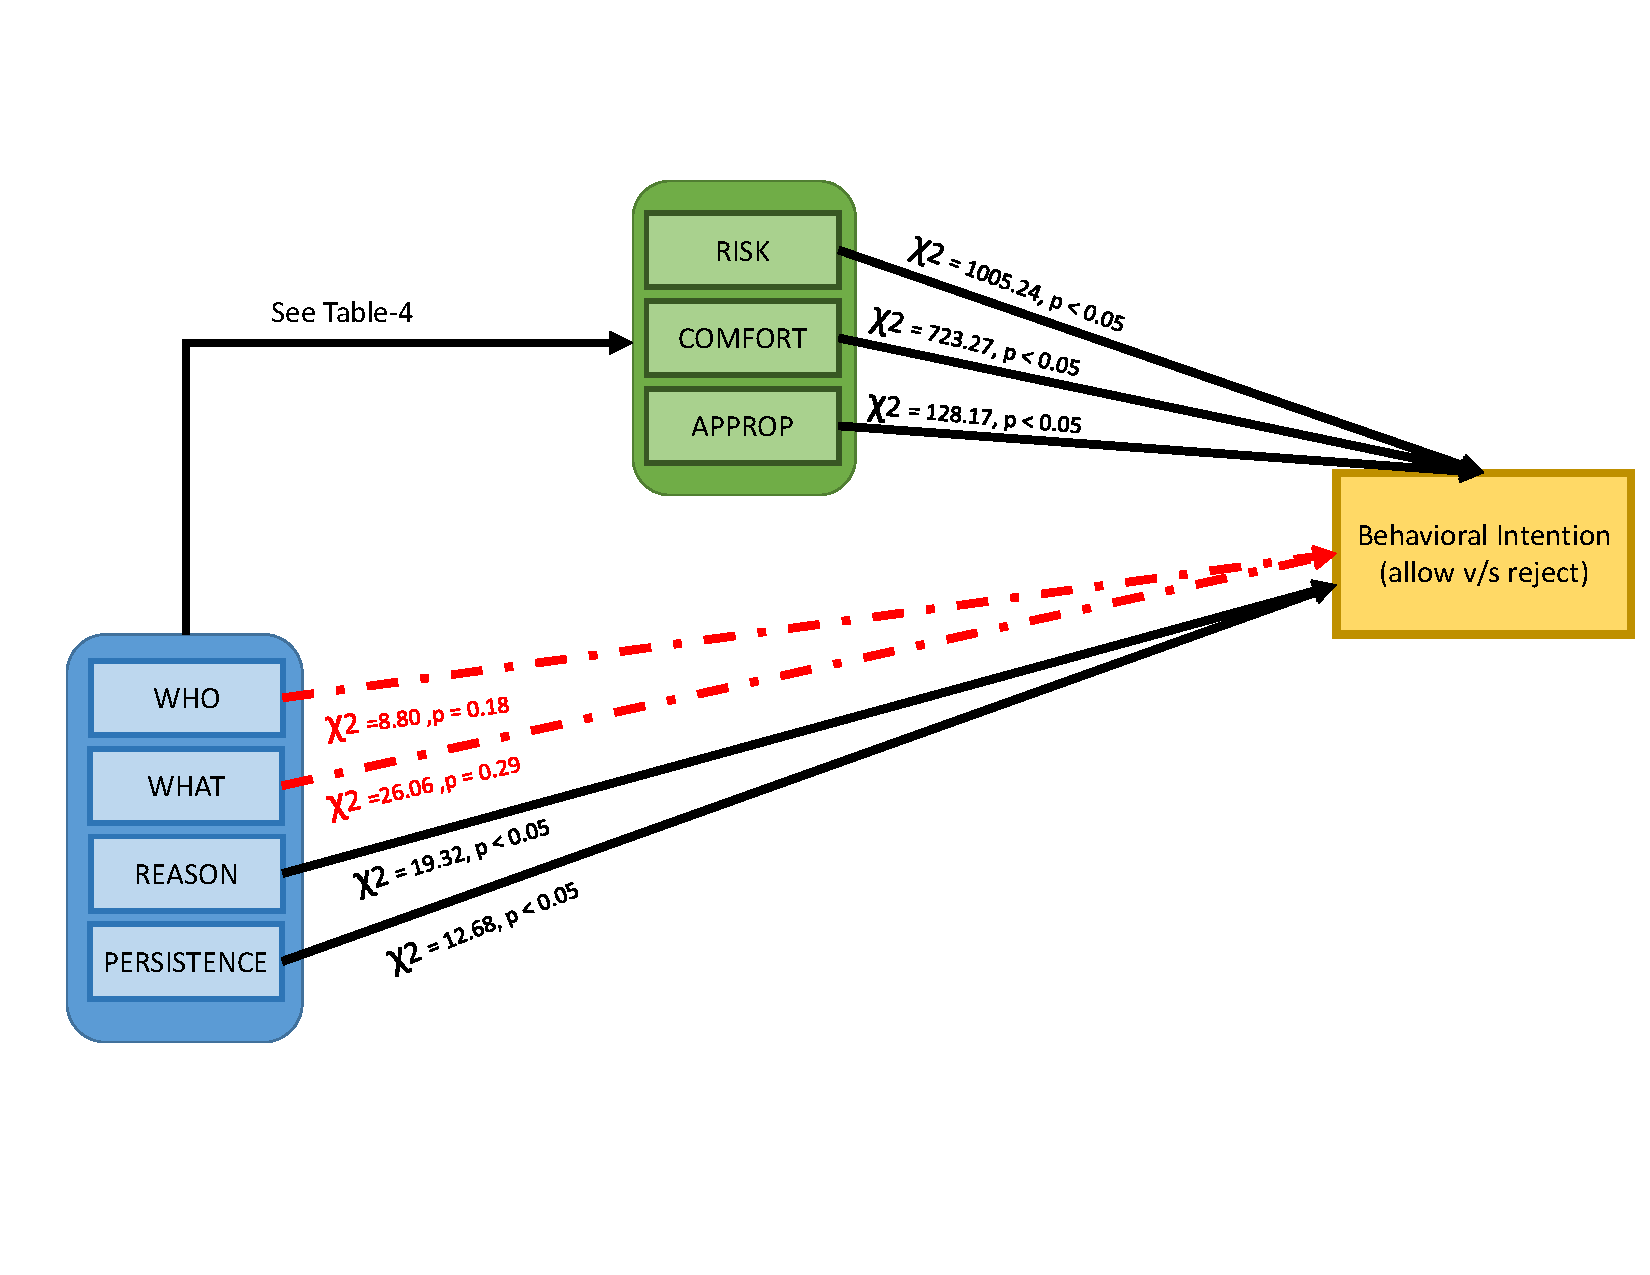
\includegraphics[width=0.45\textwidth]{figures/allow.pdf}
\caption{Mediation model of the effect of scenario parameters on participants' intention to allow/reject the scenario, mediated by attitudinal factors}
\label{fig:mediationAllow}
\end{figure}

\subsection{Discussion of Statistical Results}
Our statistical results show several patterns that can inform the development of an IoT privacy-setting interface. We find that \textbf{who} is the most important scenario parameter, and should thus end up at the top layer of our interface. People are generally concerned about IoT scenarios involving unknown and government devices, but less concerned about about data collected by their own devices. Mistrust of government data collection is in line with Li et al.'s finding regarding US audiences~\cite{li2017cross}.

\textbf{What} is the next most important scenario parameter, and its significant interaction with \textbf{who} suggests that some users may want to allow/reject the collection of different types of data by different types of recipients. Privacy concerns are higher for photo and video than for voice, arguably because photos and videos are more likely to reveal the identity of a person. Moreover, people are less concerned with revealing their age and presence, and most concerned with revealing their identity.

The \textbf{reason} for the data collection may be used as the next layer in the interface. Health and safety are generally seen as acceptable reasons. \textbf{Persistence} is less important, although one-time collection is more acceptable than continuous collection. \textbf{Where} the data is being collected does not influence intention at all. This could be an artifact of the dataset: location is arguably less prominent when reading a scenario than it is in real life.

Finally, participants' attitudes significantly (and in some cases fully) mediated the effect of scenario parameters on behavioral intentions. This means that these attitudes may be used as a valuable source for classifying people into distinct groups. Such attitudinal clustering could capture a significant amount of the variation in participants in terms of their preferred privacy settings, espcially with respect to the \textbf{who} and \textbf{what} dimensions.